\documentclass[12pt]{article}
 
\usepackage[margin=1in]{geometry} 
\usepackage{amsmath,amsthm,amssymb,bm}
\usepackage{graphicx}
%\usepackage{subcaption} % To use subfigures with subcaptions
\usepackage[caption = false]{subfig}
 
\begin{document}
  
\title{Task 2. Mesh Animation}
\author{Garoe Dorta-Perez\\
CM50245: Computer Animation and Games II}
 
\maketitle
 
\section{Introduction}

Generating a plausible mesh which is a morphing of two given meshes ...

\section{Implemented techniques}

We present two approaches to solve the mesh morphing problem. 

\subsection{Linear interpolation}

Linear interpolation is a simple and intuitive first approach.
The new position of a vertex $\mathbf{v_{it}} = \left[ v_{ix}, v_{iy}, v_{iz}\right]^T $ in an interval $t = \lbrace 0, \ldots, 1 \rbrace$ is given by

\begin{equation*}
\mathbf{v_{it}} = (1 - t) \mathbf{p_i} + t \mathbf{q_i} \quad i \in \lbrace 1, \ldots, n \rbrace,
\end{equation*}

where $n$ is the number of vertices, $\mathbf{p_i} = \left[ p_x, p_y, p_z\right]^T$ and $\mathbf{q_i} = \left[ q_x, q_y, q_z\right]^T$ are the corresponding vertices in the source and target meshes respectively.
Some meshes generated with this method are shown in Figure \ref{fig:linearInterpolation}.

\subsection{As rigid as possible interpolation}

The previous method produces distorted meshes due to its non-rigid nature.
One way to produce better results is to use a transform-based technique.
Lets define an affine transformation from $\mathbf{p_i}$ to $\mathbf{q_i}$ such that:

\begin{align*}
A \mathbf{p_i} + \mathbf{l} = \begin{pmatrix}
 a_{11} & a_{12} & a_{13} \\ 
 a_{21} & a_{22} & a_{23} \\ 
 a_{31} & a_{32}  & a_{33} 
\end{pmatrix} 
\begin{pmatrix}
 p_{ix} \\ 
 p_{iy} \\ 
 p_{iz} 
\end{pmatrix} +
\begin{pmatrix}
 l_x \\ 
 l_y \\ 
 l_z
\end{pmatrix} = \mathbf{q_i}.
\end{align*}

We have a matrix $A_{s}$ for each triangle, since there are 12 unknowns and each triangle only gives 9 equations, we add a extra point to be able to compute $A_i$.
This new point is computed as $\mathbf{p_{new}} = \mathbf{c_{tr}} + w\mathbf{n_{tr}}$, where $\mathbf{c_{tr}}$ is the triangle centroid, $w$ is the average triangle edge length and $\mathbf{n_{tr}}$ is the triangle normal. 
Since in a general mesh vertices a shared among different triangles, lets define $B_{j}$ as the actual transformation matrix, where

\begin{equation*}
E(t) = \sum_{s}^S \left \| A_s(t) - B_s(t) \right \|^2_F,
\end{equation*}

where $\left \| \cdot \right \|_F$ is the matrix Frobenius norm, and the objective is to minimize $E(t)$.
If we ignore the $l$ term, rename $\mathbf{q_i}$ to treat each vertex in individual vertex in the mesh as $\mathbf{v}_i$ the mesh, and rearrange $B$ such that

\begin{equation*}
PB_{col} = 
\begin{pmatrix}
 \mathbf{p}_i^T & \mathbf{0} & \mathbf{0} \\ 
 \mathbf{0} & \mathbf{p}_i^T & \mathbf{0}\\ 
 \mathbf{0} & \mathbf{0} & \mathbf{p}_i^T \\
  \mathbf{p}_j^T & \mathbf{0} & \mathbf{0} \\ 
 \mathbf{0} & \mathbf{p}_j^T & \mathbf{0}\\ 
 \mathbf{0} & \mathbf{0} & \mathbf{p}_j^T \\
  \mathbf{p}_k^T & \mathbf{0} & \mathbf{0} \\ 
 \mathbf{0} & \mathbf{p}_k^T & \mathbf{0}\\ 
 \mathbf{0} & \mathbf{0} & \mathbf{p}_k^T 
\end{pmatrix}
\begin{pmatrix}
b_{11} \\
b_{12} \\
b_{13} \\
b_{21} \\
b_{22} \\
b_{23} \\
b_{31} \\
b_{32} \\
b_{33}
\end{pmatrix} =
\begin{pmatrix} 
v_{ix} \\
v_{iy} \\
v_{iz} \\
v_{jx} \\
v_{jy} \\
v_{jz} \\
v_{kx} \\
v_{ky} \\
v_{kz}
\end{pmatrix} ~
\text{and} ~
P^{-1} = 
\begin{pmatrix}
\alpha_1 & 0 & 0 & \delta_1 & 0 & 0 & \lambda_1 & 0 & 0 \\
\alpha_2 & 0 & 0 & \delta_2 & 0 & 0 & \lambda_2 & 0 & 0 \\
\alpha_3 & 0 & 0 & \delta_3 & 0 & 0 & \lambda_3 & 0 & 0 \\
0 & \beta_1 & 0 & 0 & \epsilon_1 & 0 & 0 & \mu_1 & 0 \\
0 & \beta_2 & 0 & 0 & \epsilon_2 & 0 & 0 & \mu_2 & 0 \\
0 & \beta_3 & 0 & 0 & \epsilon_3 & 0 & 0 & \mu_3 & 0 \\
0 & 0 & \gamma_1 & 0 & 0 & \kappa_1 & 0 & 0 & \pi_1 \\
0 & 0 & \gamma_2 & 0 & 0 & \kappa_2 & 0 & 0 & \pi_2  \\
0 & 0 & \gamma_3 & 0 & 0 & \kappa_3 & 0 & 0 & \pi_3
\end{pmatrix},
\end{equation*}

then we have that $B = P^{-1}V$.
We would have the above system for each triangle in the mesh, with its own $P$ and $B$ matrices.  
Writing explicitly the Frobenius terms in $E(t)$, and expressing $B$ as a linear combination of $\mathbf{v}_i$, we get

\begin{align*}
E(t) &= \lbrace a_{11}^2 + a_{12}^2 + \ldots + a_{33}^2 + \alpha_1^2 v_{1x}^2 + \ldots + \pi^2 v_{3z}^2 - 2 a_{11} \alpha_1 v_{1x} \\
& - 2 a_{11} \delta_1 v_{2x} - 2 a_{11} \lambda_1 v_{3x} - \ldots - 2 a_{33} \pi_3 v_{3z} + 2 \alpha_1 v_{1x} \delta_1 v_{2x} \\ 
& + 2 \alpha_1 v_{1x} \lambda_1 v_{3x} + \ldots + 2 \kappa_3 v_{2z} \pi_3 v_{3z} \rbrace_{j = 1} + \ldots + \lbrace \cdots \rbrace_{j = J},
\end{align*}

where we have a $\lbrace \cdots \rbrace_j$ for each triangle.
Predetermining the transformation of $\mathbf{v_1}$, and setting 
$\mathbf{u}^T = \begin{pmatrix} 1, v_{2x}, v_{2y}, v_{2z}, \ldots, v_{mx}, v_{my}, v_{mz} \end{pmatrix}$, where $m$ is the number of vertices, we can stack the terms in a quadratic matrix form 

\begin{equation*}
E(t) = \mathbf{u}^T  \begin{pmatrix}
c & \mathbf{g^T} \\
\mathbf{g} & H
\end{pmatrix} \mathbf{u},
\end{equation*}

where $c$ are the constant coefficients, $\mathbf{g}$ is a vector with the terms linear on $a_i$ and $H$ is matrix with the quadratic and mixed terms.
Note that the terms involving $\mathbf{v}_1$ are are treated differently since it is not an unknown.

\begin{figure}
\subfloat[fig 3]{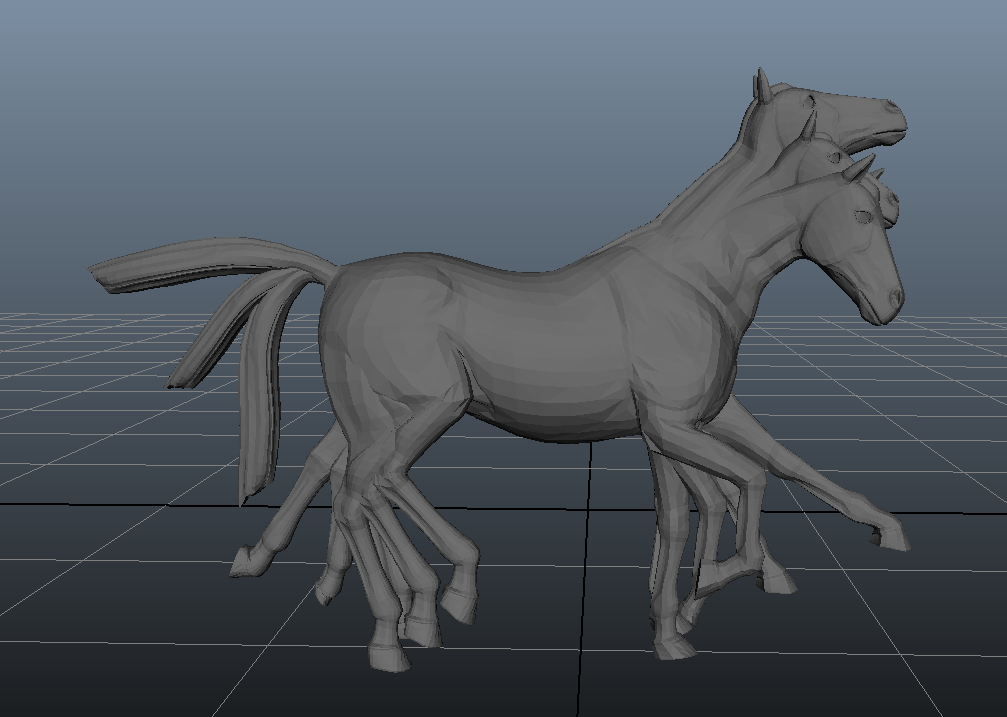
\includegraphics[width = 3in]{images/linearInterpolation1}}
\subfloat[fig 4]{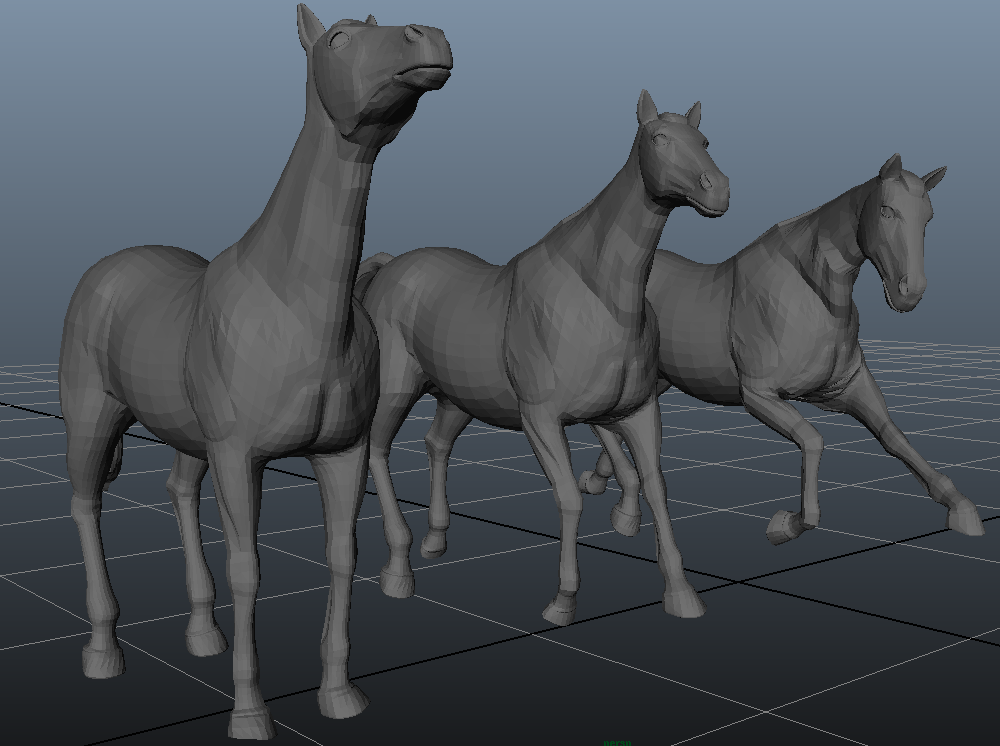
\includegraphics[width = 3in]{images/linearInterpolation2}}\\
\subfloat[fig 1]{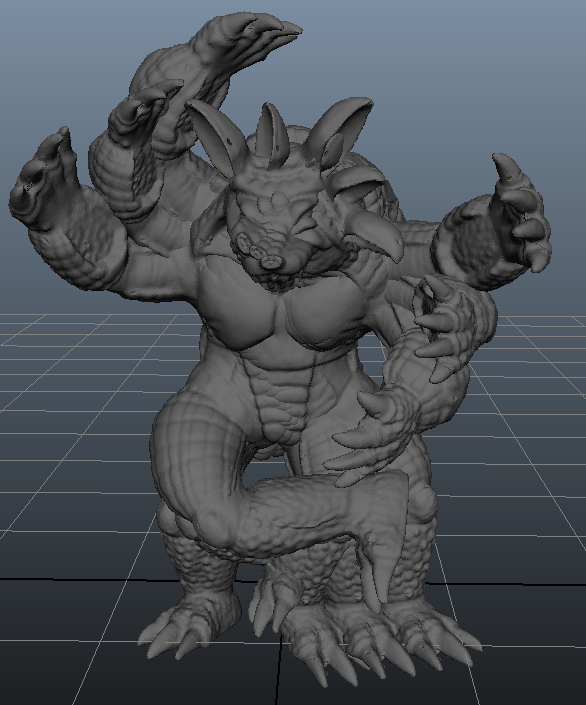
\includegraphics[width = 1.8in]{images/armadillo2}}
\subfloat[fig 2]{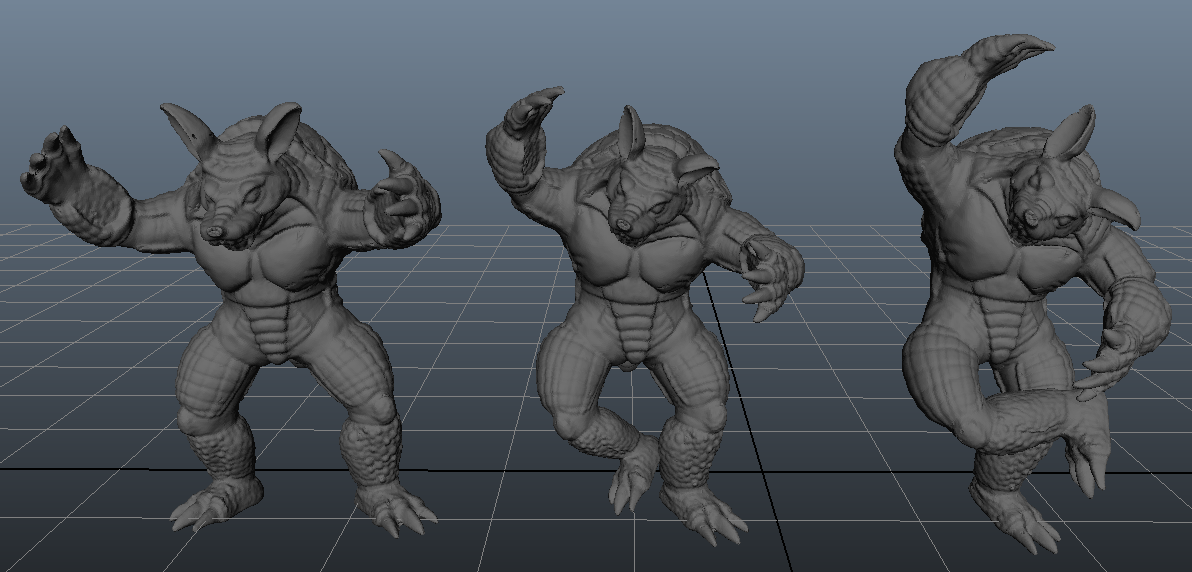
\includegraphics[width = 3.3in]{images/armadillo1}} 
\caption{Horse and armadillo meshes, morphed mesh is in the middle.}
\label{fig:linearInterpolation}
\end{figure}

\end{document}

